% Created 2022-04-19 Tue 14:00
% Intended LaTeX compiler: pdflatex
\documentclass[smaller]{beamer}\usepackage{listings}
\usepackage{color}
\usepackage{amsmath}
\usepackage{array}
\usepackage[T1]{fontenc}
\usepackage{natbib}
\lstset{
keywordstyle=\color{blue},
commentstyle=\color{red},stringstyle=\color[rgb]{0,.5,0},
literate={~}{$\sim$}{1},
basicstyle=\ttfamily\small,
columns=fullflexible,
breaklines=true,
breakatwhitespace=false,
numbers=left,
numberstyle=\ttfamily\tiny\color{gray},
stepnumber=1,
numbersep=10pt,
backgroundcolor=\color{white},
tabsize=4,
keepspaces=true,
showspaces=false,
showstringspaces=false,
xleftmargin=.23in,
frame=single,
basewidth={0.5em,0.4em},
}
\usepackage{natbib, dsfont, pgfpages, tikz,amssymb, amsmath,xcolor}
\bibliographystyle{plain}
% New operators and commands
\newcommand{\Z}{\mathbb{Z}}
\newcommand{\Q}{\mathbb{Q}}
\newcommand{\R}{\mathbb{R}}
\newcommand{\N}{\mathbb{N}}
\newcommand{\C}{\mathbb{C}}
\renewcommand{\S}{\mathbb{S}}
\newcommand{\blank}{\makebox[1ex]{\textbf{$\cdot$}}}
\newcommand\independent{\protect\mathpalette{\protect\independenT}{\perp}}
\def\independenT#1#2{\mathrel{\rlap{$#1#2$}\mkern2mu{#1#2}}}
\renewcommand{\phi}{\varphi}
\renewcommand{\epsilon}{\varepsilon}
\newcommand*\diff{\mathop{}\!\mathrm{d}}
\newcommand{\weakly}{\rightsquigarrow}
\newcommand\smallO{
  \mathchoice
    {{\scriptstyle\mathcal{O}}}% \displaystyle
    {{\scriptstyle\mathcal{O}}}% \textstyle
    {{\scriptscriptstyle\mathcal{O}}}% \scriptstyle
    {\scalebox{.6}{$\scriptscriptstyle\mathcal{O}$}}%\scriptscriptstyle
}
\newcommand{\midd}{\; \middle|\;}
\newcommand{\1}{\mathds{1}}
\usepackage{ifthen} %% Empirical process with default argument
% \newcommand{\G}[1][]{%
%    \ifthenelse{ \equal{#1}{} }
%       {\ensuremath{\mathbb{G}_n}}
%       {\ensuremath{\mathbb{G}_{#1}}}
% }
% New version:
\newcommand{\G}[2][n]{
{\ensuremath{\mathbb{G}_{#1}}{\left[#2\right]}}
}
\DeclareMathOperator*{\argmin}{\arg\!\min}

% New operators for consistent notation
\newcommand{\V}{\mathrm{Var}} % variance
\newcommand{\measure}[1]{\mathrm{{#1}}} % measure
% \newcommand{\measure}[1]{\textnormal{\textbf{{#1}}}} % measure
\newcommand{\m}[1]{\measure{#1}} % measure shortcut
\newcommand{\eqd}{\stackrel{d}{=}} % equality in distribution
\newcommand{\arrowP}{\xrightarrow{\; \m{P} \;}} % convergence in probability
\newcommand{\leb}{\lambda} % the Lebesgue measure
\newcommand{\T}{\top} % transpose

\usepackage{xargs}
% Make it easy to change counterfactual notation:
\newcommandx{\cf}[4][3={}, 4={}]{
  % \ifthenelse{ \equal{#4}{} }
  % {{#1^{#2}}(#3)}
  {\ifthenelse{ \equal{#3}{} }
    {{#1^{#2}}_{#4}}
    {{#1^{#2}}_{#4}(#3)}}
}

% Easily change notation:
\DeclareMathOperator{\TT}{\Psi} % target parameter
\newcommand{\lp}{\mathcal{L}_{\P}^2} % shortcut for lp2 space
\newcommand{\empmeas}{\hat{\mathbb{P}}_n} % empirical measure
\DeclareMathOperator{\E}{\mathbb{E}} % expectation
\renewcommand{\P}{\m{P}} % probability
\newcommand{\ic}{\mathrm{IF}} % influence curve
\setbeamertemplate{footline}[frame number]
\beamertemplatenavigationsymbolsempty
\usepackage{appendixnumberbeamer}
\setbeamercolor{gray}{bg=white!90!black}
\setbeamertemplate{itemize items}{$\circ$}

\renewcommand*\familydefault{\sfdefault}
\itemsep2pt
\usepackage[utf8]{inputenc}
\usepackage[T1]{fontenc}
\usepackage{graphicx}
\usepackage{longtable}
\usepackage{wrapfig}
\usepackage{rotating}
\usepackage[normalem]{ulem}
\usepackage{amsmath}
\usepackage{amssymb}
\usepackage{capt-of}
\usepackage{hyperref}
\usetheme{default}
\author{Anders Munch \& Thomas Gerds}
\date{April 25, 2022}
\title{Project in Biostatistics: Hyperparameter optimization}
\begin{document}

\maketitle
\begin{frame}[label={sec:org8237656}]{Outline of the setting}
Let $\mathcal{P}$ be a collection of probability measures over $\R^{d+2}$, so that
$O \sim P \in \mathcal{P}$, with $O = (Y, A, X)$, $Y\in \R$, $A\in \R$, and $X \in \R^d$.

\vfill

We consider estimation of a parameter $\theta \colon \mathcal{P} \rightarrow \Theta$, where $\Theta$
is either a \textbf{high-} or a \textbf{low-dimensional} space:

\vfill

\begin{enumerate}
\item Risk prediction model: For some suitable function space \(\mathcal{F}\), the parameter of interest
is \(\nu \colon \mathcal{P} \rightarrow \mathcal{F}\), \[\nu(P) = f, \text{ for } f(x, a) = \E_P[Y
   \mid X=x, A=a]. \]
\item Low-dimensional (causal) target parameter, for instance the average treatment effect: The
parameter of interest is \(\Psi \colon \mathcal{P} \rightarrow \R\), \[\Psi(P) = \E_P{\left[ \E_P[Y
   \mid X, A=1] - \E_P[Y \mid X, A=0] \right]}. \]
\end{enumerate}
\end{frame}

\begin{frame}[label={sec:org345616e}]{Data}
You will work with a random subset of the data described in \cite{wikkelso2014prediction}. The
dataset contains data from 48,272 Danish women who gave birth twice. The main outcome is a binary
variable called PPH which indicates if the woman had a postpartum haemorrhage (heavy bleeding)
during the second delivery.

\vfill

\begin{block}{High- and low-dimensional inference problems}
\begin{enumerate}
\item Predicting the risk of PPH at second delivery.
\item Estimating the causal effect of a planned cesarian section on PPH.
\end{enumerate}
\end{block}
\end{frame}

\begin{frame}[label={sec:org9f77f7c}]{Hyperparameter and model selection/construction}
Estimation of \(\nu\) is a well-studied problem. Many (machine) learning approaches depend on one or
more hyperparameters that has to be tuned. We want to examine how to do this properly, and what the
practical effects are of the different possible approaches.

\vfill

\begin{block}{Examples of things to consider}
\begin{itemize}
\item How do we evaluate the performance of a candidate model?
\item Do we select a single candidate model as our final model, or do we combine the candidate models
into one? One approach is the Super Learner \citep{van2011targeted,HoffmanBlog}.
\item What kind of theoretical guarantees do we get when using cross-validation to select/construct a model?
\item How does the different approaches play out in practice?
\end{itemize}
\end{block}
\end{frame}

\begin{frame}[label={sec:org4f946cd}]{Target parameter and causal inference}
\begin{block}{Target parameter}
By explicitly defining a parameter of interest as an answer to a concrete scientific question, we
ensure that we can draw relevant and meaningful conclusions from our statistical analysis.
\end{block}

\begin{block}{High-dimensional nuisance parameter}
By allowing high-dimensional nuisance parameters we avoid having to make unrealistic model
assumptions.
\end{block}

\begin{block}{Causal inference}
One example is the average treatment effect, \[\Psi(P) = \E_P{[\nu(X, 1) -\nu(X, 0)]}, \quad
\nu=\nu(P) \in \mathcal{F}. \]

\begin{itemize}
\item How do we formalize a causal question?
\item Which assumptions are needed for the above parameter to have a causal interpretation?
\item How likely are these assumptions to hold for the data at hand?
\end{itemize}
\end{block}
\end{frame}

\begin{frame}[label={sec:org8f54092}]{Targeted inference and hyperparameter selection}
Finding a good estimator \(\hat\nu\) of \(\nu\) \alert{does \emph{not} necessarily provide a good plug-in estimator
of \(\Psi\)}! \(\rightarrow\) targeted learning and debiased ML
\citep{van2006targeted,van2011targeted,chernozhukov2018double,kennedy2022semiparametric}.

\hfill

Let \(\hat\nu_{\lambda}\) be the ridge regression estimator of \(\nu\) with penalty parameter \(\lambda\).
Let \(\hat\Psi_{\lambda}\) denote the plug-in estimator of \(\Psi\) based on \(\hat\nu_{\lambda}\), i.e.,
\small
\begin{equation*}
  \hat\Psi_{\lambda} = \frac{1}{n}\sum_{i=1}^{n}
  \left\{
    \hat{\nu}_{\lambda}(X_i, 1)- \hat{\nu}_{\lambda}(X_i, 0)
\right\}.
\end{equation*}


\begin{center}
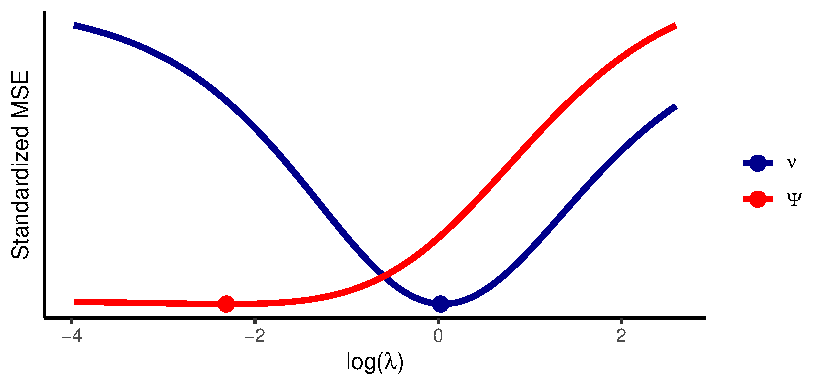
\includegraphics[width=.9\linewidth]{./fig-nuisance-target-tuning.pdf}
\end{center}
\end{frame}

\begin{frame}[label={sec:orgd13ceb5}]{References}
\small\bibliography{../latex-settings/default-bib.bib}
\end{frame}
\end{document}